\documentclass[12pt,letterpaper]{article}
\usepackage{pdfpages}
\usepackage{fancyhdr}
\usepackage[colorlinks=true, urlcolor=blue, linkcolor=blue]{hyperref}
\usepackage{graphicx}
\usepackage[top=1.4in, left=0.5in, right=0.5in, bottom=0.8in]{geometry}
\usepackage[T1]{fontenc}
\usepackage{helvet}
\pagestyle{fancy}
\renewcommand{\headrulewidth}{0pt}
\renewcommand{\footrulewidth}{0pt}
\setlength{\parindent}{0em}
\setlength{\parskip}{1em}


\fancyfoot[C]{\setlength{\unitlength}{1in}\begin{picture}(5,0)\put(-1.8,-1){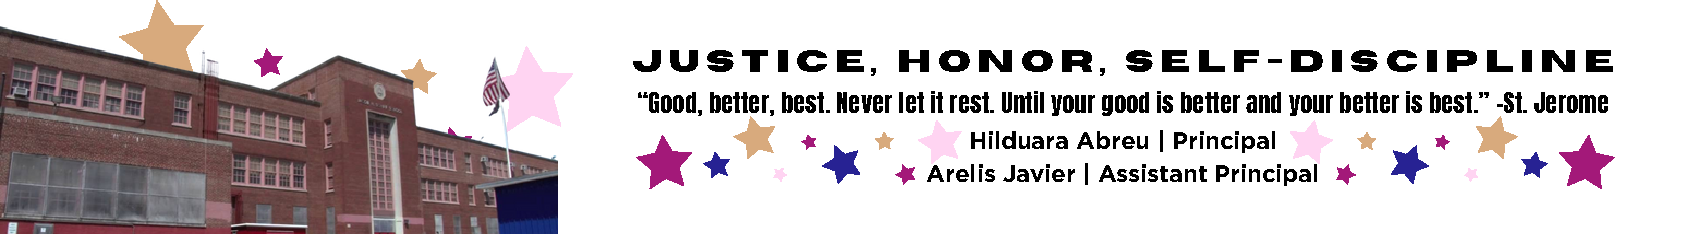
\includegraphics[width=8.8in,height=1.3in]{logo-1}}\end{picture}}
\fancyhead[C]{\setlength{\unitlength}{1in}\begin{picture}(5,0)\put(-1.9,-1){
\includegraphics[width=8.9in,height=1.3in]{logo-2}}\end{picture}}

\pagenumbering{gobble}
\addtolength{\evensidemargin}{-2in}
\addtolength{\topmargin}{-0.5in}
\addtolength{\textwidth}{0in}
%%%%%%%%%%%%%%%%%%%%%%%%%%%%%%%%%%%%%%%%%%%%%%%%%%%%%%%%%%%%%%%%%%

\begin{document}
\vspace*{0.5in}
Date: \href{https://www.ps192.org/apps/bbmessages/show_bbm.jsp?REC_ID=139439}{September 14, 2023} 

\textbf{Subject: School Year 2023-24 | PS 192 Visitor and Safety Guidelines and Procedures}

Dear Parents and Guardians,

We are pleased to present the guidelines and procedures for our esteemed institution, Jacob H. Schiff/P.S. 192. These guidelines and procedures have been meticulously designed to prioritize the safety and security of all individuals—our valued students, dedicated staff, and respected visitors—while fostering an environment that is welcoming and inclusive. We sincerely appreciate your cooperation in adhering to these essential protocols.
\begin{itemize}
	\item Visitor Registration:
		\begin{itemize}
		\item Upon Arrival: All visitors, including parents, guardians, 
		volunteers, contractors, and esteemed guests, are kindly requested to
		enter the school premises through the main entrance and proceed to the
		safety agent desk for registration.
		\item Warm Welcome: Our School Safety Agent or designated school staff 
		will warmly welcome all visitors, inquire about the purpose of your
		visit, and request a valid photo ID.
		\item Identification: To ensure security, visitors must present a valid
		form of identification, such as a driver's license, government-issued
		ID, foreign or US passport, or consulate identification card.
		Subsequently, visitors will be given an identification sticker, which
		must be prominently displayed throughout their visit. The School Safety
		Agent will assist in issuing the identification sticker.
		\item Assistance Notification: Once the School Safety Agent or 
		designated school staff completes the registration process, they will
		notify the parent coordinator by calling X1190. This will facilitate
		further assistance for the visitor, whether waiting in the lobby or the
		auditorium.
		\item Departure Protocol: Visitors are kindly requested to sign out with
		the School Safety Agent or designated school staff upon leaving the 
		building. The identification sticker should be returned; the main 
		entrance is the recommended exit point.
		\end{itemize}
	\item Language Assistance:
		\begin{itemize}
		\item When a visitor does not communicate in English, our School Safety Agent (SSA) or designated school staff member will try to identify the visitor's language. A multi-language poster displayed at the safety desk will be used for language identification. Once the language is ascertained, the visitor will be directed to the parent coordinator for further assistance. In cases where we need staff proficient in the visitor's language on-site, the parent coordinator will engage the DOE's Over-the-Phone Interpretation Unit to arrange an on-demand interpreter.
		\end{itemize}
\pagebreak
\vspace*{1.5cm}
	\item Appointments:
		\begin{itemize}
		\item Open Door Policy: Every Tuesday from 2:20-3:00 p.m., ALL staff members are available for meetings with parents/caregivers.
		\item Scheduled Visits: We encourage non-emergency visits to be scheduled whenever possible to ensure that staff members are available to meet with visitors and minimize disruption to instructional time. Visitors and staff can schedule appointments through various channels, including Classdojo, staff direct email, our school website, or contact the parent coordinator.
		\item Visitor Arrival: Upon arriving for a scheduled appointment, visitors are kindly requested to follow the same entrance and registration process outlined above.
		\end{itemize}
	\item Escort and Supervision:
		\begin{itemize}
		\item Visitor Escort: For added security, a designated staff member will escort visitors to and from their intended destination within the school premises, including classrooms, offices, the library, the gym, and other shared spaces.
		\item Supervised Contact: Visitors should interact with students only if expressly authorized by school administration or as part of a pre-approved program or event.
		\end{itemize}
	\item Confidentiality and Privacy:
		\begin{itemize}
		\item Media and Privacy: To uphold our students and staff members' privacy and confidentiality, visitors are kindly requested not to take photographs or record videos while on school premises.
		\item Respect for Privacy: Any personal information or observations made during the visit should not be shared without appropriate consent or authorization from the NYC DOE.
		\end{itemize}
	\item Safety Drills:
		\begin{itemize}
		\item Throughout the academic year, we conduct safety drills to ensure that students and staff are well-prepared to respond effectively in emergencies. These drills are essential for the safety and security of our school community and include:
			\begin{itemize}
			\item 12 Fire Drills: Conducted bi-weekly from September to December 31, 2023, and monthly after that.
			\item 4 Lockdown Drills: Conducted every other month.
			\item 2 Bus Emergency Drills: Conducted at the beginning of the school year and the start of the second semester (February 2024).
			\end{itemize}
		\end{itemize}
\end{itemize}
\pagebreak
\vspace*{1.5cm}
By faithfully following these visitor guidelines and procedures, we collectively contribute to our esteemed school community's safety, security, and well-being. If you have any questions or require further clarification, please do not hesitate to contact us or contact Ms. Rijo at 646-745-0150 or 212-775-9560 X1190. Your unwavering commitment and support are pivotal in maintaining a positive and secure learning environment. Additional assistance is also available through our website or WhatsApp.

Once again, we extend our heartfelt gratitude for your cooperation and dedication to our shared mission.

In Unity,


\includegraphics[width=0.2\textwidth]{hil_signature}

\textbf{Hilduara Abreu}

\textbf{Principal}

\textit{The School of Joyful Learning!}

\url{www.ps192.org}

\end{document}
